\section*{Introduccion}

Una ataguia es una estructura temporal utilizada para drenar zonas cubiertas de agua, de este modo, es posible construir en terrenos
que de otra forma serian inaccesibles \textbf{\cite{madanayaka2018}}. Hay varios factores importantes a determinar al momento de diseñar
una ataguia, como por ejemplo el caudal de infiltracion, las presiones de poros, estabilidad de la estructura y por sobre todo la licuefaccion
y su factor de seguridad (FS). Este ultimo fenomeno ocurre cuando las presiones de poros alcanzan tal punto, que las tensiones internas efectivas
entre las particulas de suelo pierden efectividad, y en consecuencia, la mescla entre agua y sedimentos actua como un fluido \textbf{\cite{sumer2009}}
\\ \\
El presente proyecto tiene como objetivo el estido y analisis de 3 ataguias distintas, donde se buscara evaluar sus distintas caracteristicas utilizando 
calculos manuales a travez de python, un solver mediante diferencias finitas y una maqueta a escala. De esta forma, se buscara analizar la efectividad
de cada metodo de analisis, ademas, de una comparacion directa entre los resultados obtenidos.
\\ \\
En los calculos manuales, se utilizo la Ley de Darcy, ademas de las diferentes ecuaciones nesesarias para determinar una red de flujo teoricamente. De esta forma, 
se calculo parametros como el caudal de infiltracion o la prescion de poros a lo largo de toda la estructura.
\\ \\
Posterirmente, se desarrollo un solver mediante diferencias finitas, el cual es un metodo numerico utilizado para calcular diferencias de potenciales en grillas 2D o 3D \textbf{\cite{zhang2005}}.
De esta menera, y determinando que el fluoj va de un potencial mayor a uno menor, se pueden obtener las redes de flujos y asi los distintos parametros nesesarios.
\\ \\
Finalmente se realizo un modelo a escala, donde se simulo la ataguia ademas de una falla por licuefaccion. Ademas, se busco calibrar el modelo computacional en base a los datos obtenidos del modelo real, 
determinando asi, que tan efectivo es el calculo numerico, en comparacion con la realidad.
\\ \\
El modelo base utilizado a lo largo del informe es el siguiente:

\begin{figure}[H]
    \centering
    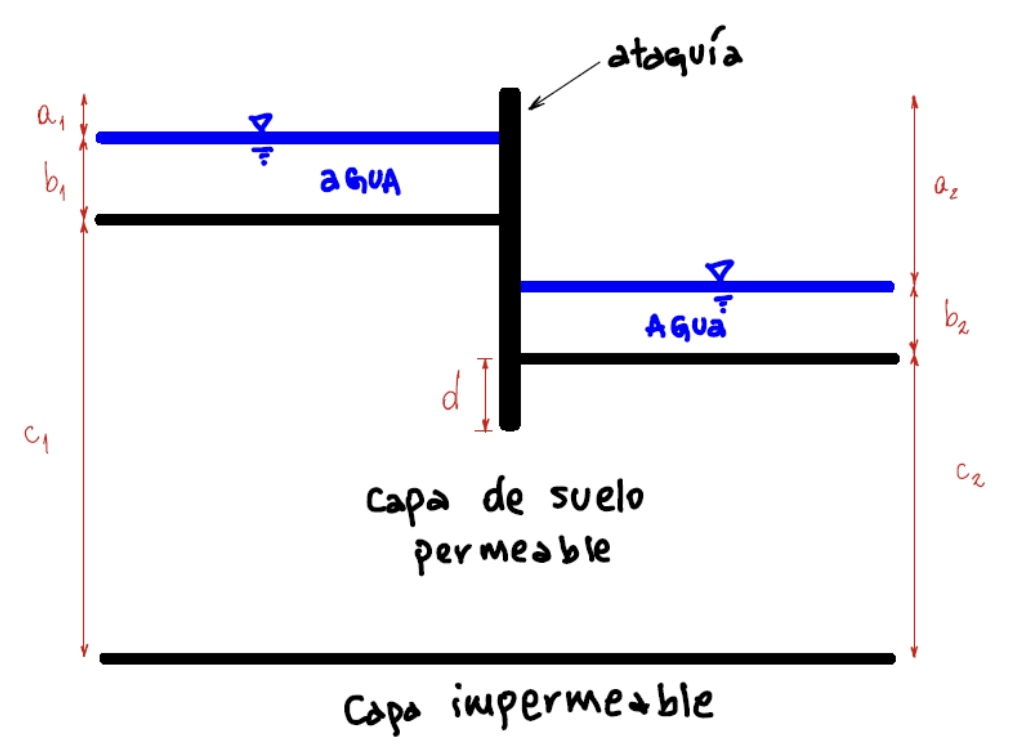
\includegraphics[width=0.45\textwidth]{FOTOS/modelo_base.png}
    \caption{Modelo Base}
    Fuente: Guia de Proyecto
    \label{fig:modelo_base}
\end{figure}

Las medidas para los distintos casos se encuentran en la tabla \textbf{\ref{tab:medidas}}.

